\documentclass[tikz,border=10pt]{standalone}
\usepackage{pgfplots}
\pgfplotsset{compat=1.18}
\begin{document}
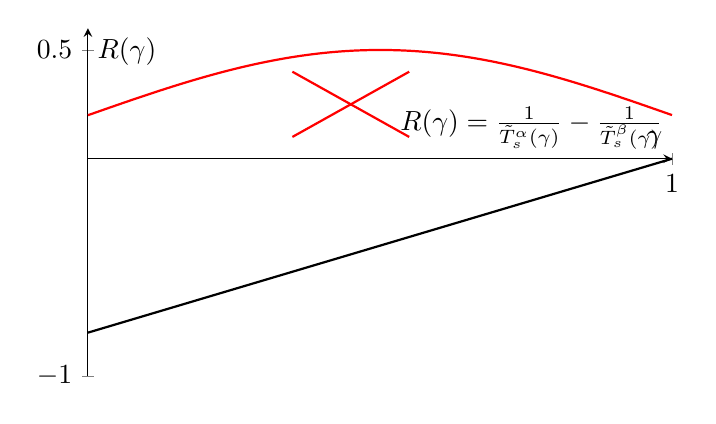
\begin{tikzpicture}
\begin{axis}[
    width=9cm,
    height=6cm,
    xmin=0, xmax=1,
    ymin=-1, ymax=0.6,
    axis lines=middle,
    xlabel={$\gamma$},
    ylabel={$R(\gamma)$},
    xtick={0,1},
    ytick={-1,0,0.5},
    domain=0:1,
    samples=100,
    clip=false
]
\addplot[black,thick] {-0.8 + 0.8*x};
\addplot[red,thick] {0.2 + 0.3*sin(deg(3.14*x))};
\node[anchor=south east] at (axis cs:1,0) {$R(\gamma)=\frac{1}{\tilde{T}_s^{\alpha}(\gamma)}-\frac{1}{\tilde{T}_s^{\beta}(\gamma)}$};
% Cross out the red curve
\draw[red,thick] (axis cs:0.35,0.4) -- (axis cs:0.55,0.1);
\draw[red,thick] (axis cs:0.35,0.1) -- (axis cs:0.55,0.4);
\end{axis}
\end{tikzpicture}
\end{document}
